\subsection{Comparing neural geometries in shape space}

% Before turning to experimental data, we show with simulated data how challenging it is to unveil structure across systems and how a proper metric can be leveraged to unveil such structure. 

We start by laying out a rigorous framework to compare neural geometries across scales, proceed with showing in simulations how structure at the neuron level does not imply structure at another scale and finally use shape spaces to infer structure across regions and individuals in psychophysiological recordings from many regions and animals. Consider a set of neural recordings collected across $K$ biological systems---for example, $K$ different animals, $K$ behavioral sessions from the same animal, or recordings from $K$ different brain regions (\textbf{Fig.}~\ref{fig:schematic}a).
The activity of each neural system is recorded at $M$ measurement points, corresponding to different experimental conditions or time points.
For example, neural responses could be measured in response to $C$ conditions (e.g. distinct sensory stimuli or trained motor actions) over $T$ time points per condition.
This would result in a total of $M = C\,T$ measurements.
To simplify the exposition, we will assume that each neural population is composed of $N$ neurons\footnote{This assumption is typically violated in practice, but our approach is easy to adapt to unequal neural populations (see \textit{Methods} and \cite{harvey2024duality}).}. In this setting, the data collected from $K$ neural systems are represented by a set of $N \times M$ matrices, $\mbX_1, \mbX_2, \dots, \mbX_K$.
Each row corresponds to a neuron's tuning curve across the $M$ measurement points and each column corresponds to an $N$-dimensional population response to one of the experimental measurements.
\textbf{Fig.}~\ref{fig:schematic}b illustrates an example where the measurements span a 1-dimensional space, resulting in a 1-dimensional, smooth manifold structure within the neural firing rate space.

\begin{figure}
    \centering
    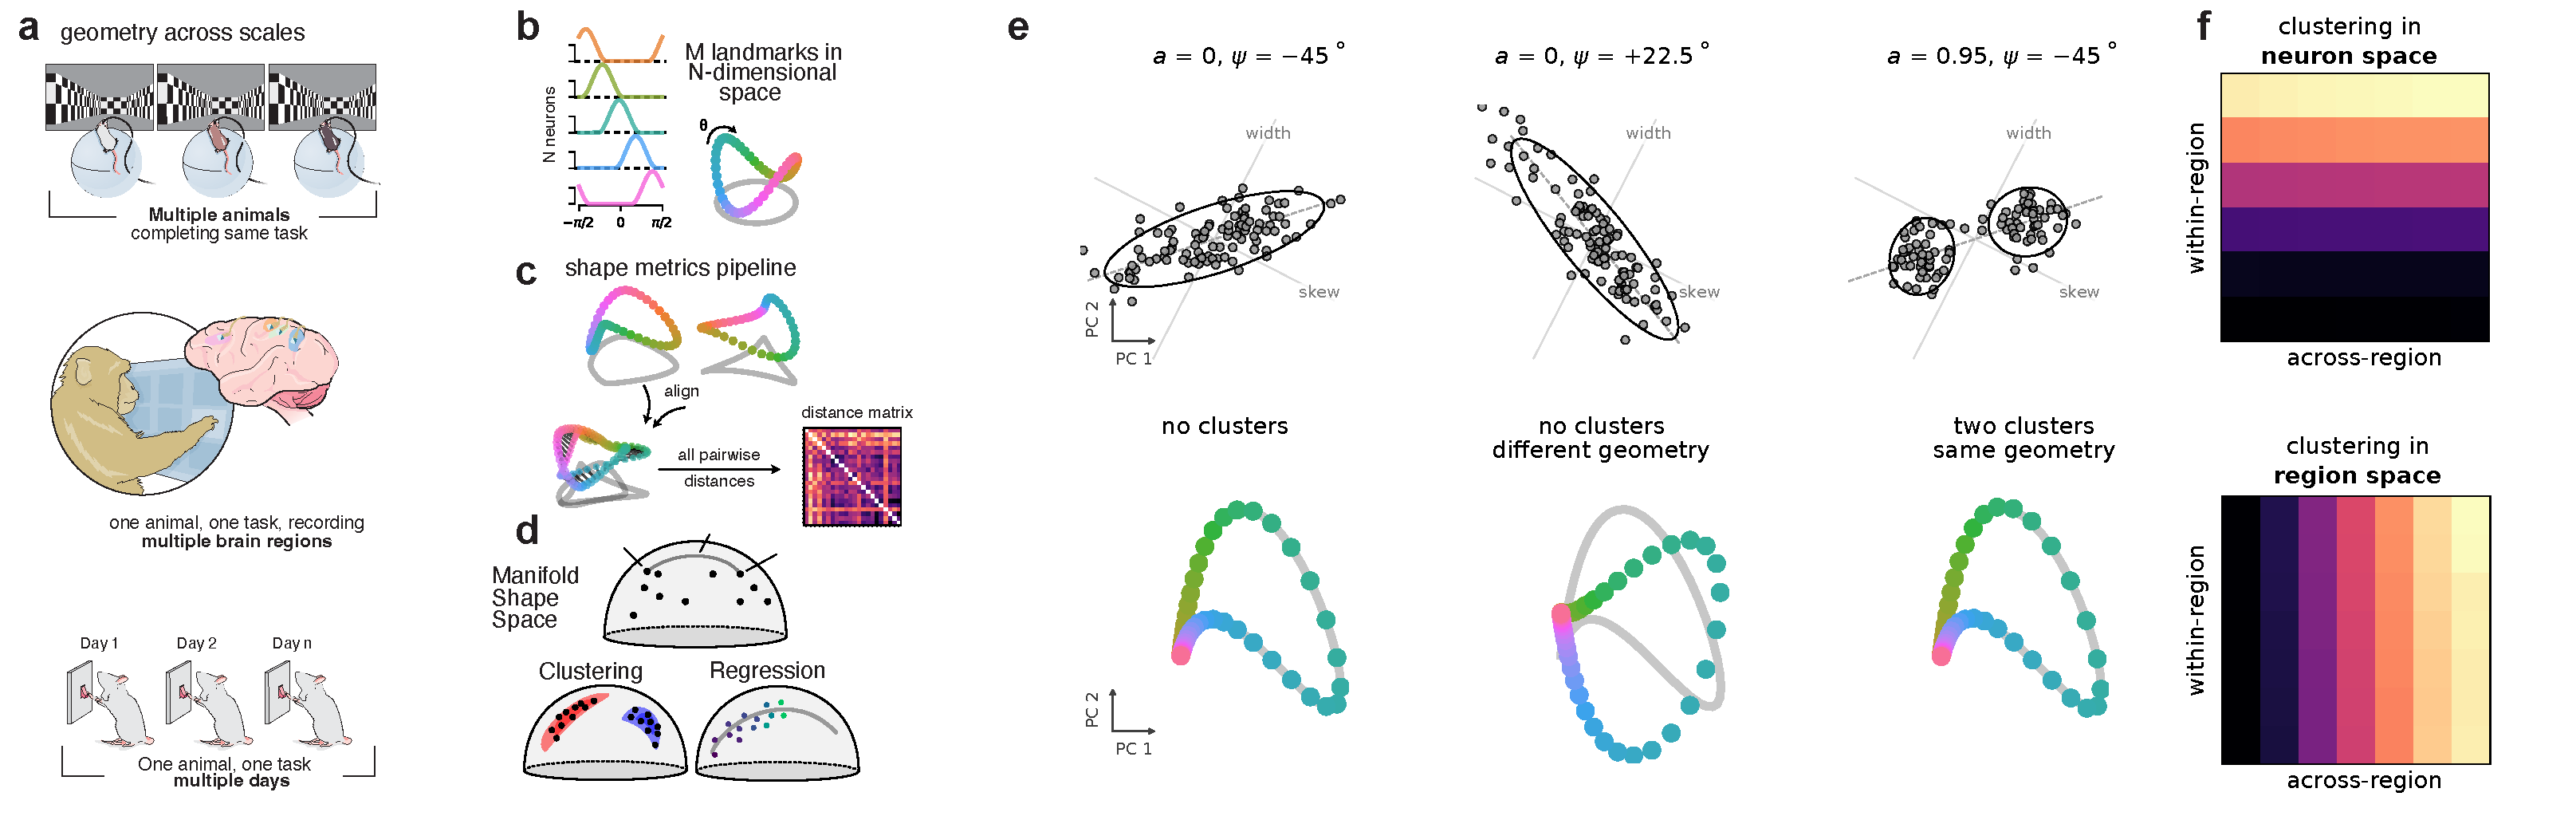
\includegraphics[width=1\textwidth]{content/figures/netrep-journal-figure-1b.pdf}

       \caption{\textbf{A geometric framework for comparing neural populations across scales.}
     \textbf{a.} Shape metrics can be leveraged to compare representations across animals, regions or different time periods from the same animal. \textbf{b.} Example population activity measured across $M$ conditions and $N$ neurons in a simulated experiment parameterized by a periodic 1D variable, $\theta$ (e.g. head direction). Smooth tuning curves, \textit{left}, can be viewed as a smooth manifold, \textit{right}, in $N$-dimensional firing rate space. Color code denotes values of $\theta$. \textbf{c.} The goal of our framework isto compute a distance function $d(X_i,X_j)$, which we define as the dissimilarity between two manifolds $X_i, X_j$ after alignment. \textbf{d.} The set of possible manifolds and the distance function together define a \textit{metric space}. The properties of these metric spaces allow us to leverage existing methods, such as clustering and regression with rigorous theoretical guarantees. \textbf{e} Simulation of 3 regions, $N = 100$ neurons each where population geometry and clusters in neuron space are decoupled. Every neuron is a point in a two-dimensional space of tuning shapes (skew, width), shown here as the first two principal components of the neurons $\times$ conditions matrix, with the skew and width directions recovered by regression (grey axes). \textit{Left}, a region without any clusters. \textit{Middle}, another region without any clusters but a rotated cloud in width-skew space leads to a different geometry, bottom. \textit{Right}, a region with the same overall orientation as on the left, but with two clusters, leads to a similar geometry. Bottom row, each region's population manifold, with the left region's manifold repeated in grey behind all three after optimal alignment. \textbf{f.} Clustering analyses over a two-dimensional design in which within-region clustering (vertical) and across-region clustering (horizontal) are varied independently; colour is $z$ against each method's own null. Pooling neurons responds to within-region clustering and is flat along the other axis; the region-space test does the reverse.
    }
        \label{fig:schematic}
\end{figure}

We leverage the \textit{Procrustes shape distance} \parencite{schonemann1966generalized} as a convenient way to quantitatively compare neural geometries (\textbf{Fig.} \ref{fig:schematic}c).
This distance is calculated as
\begin{equation}
\label{eq:procrustes-distance}
d(\mbX_i, \mbX_j) = \min_{\mbQ \in \cO(N)} \Vert \mbQ \mbX_i - \mbX_j \Vert_F
\end{equation}
where $\cO(N)$ is the set of $N \times N$ orthogonal matrices.
Intuitively, $\mbQ$ encodes the optimal rotation and reflection that minimizes the sum of squared residuals between the two neural manifolds\footnote{We assume that each neuron's tuning curve has been pre-processed to be mean centered (i.e. rows of $\mbX_i$ and $\mbX_j$ have mean zero), so that the rotational alignment is applied around each manifold's center of mass.}. 

The Procrustes distance satisfies two key properties of \textit{symmetry}, $d(\mbX_i, \mbX_j) = (\mbX_j, \mbX_i)$, and the \textit{triangle inequality}, $d(\mbX_i, \mbX_j) \leq (\mbX_j, \mbX_k) + (\mbX_k, \mbX_j)$, which permits us to envision the collection of neural geometries, represented as the matrices $\mbX_1, \mbX_2, \dots, \mbX_K$, as $K$ discrete points in a common ``shape space'' of possible geometries (\textbf{Fig.} \ref{fig:schematic}d)
Clusters of points within this space correspond to neural systems with similar manifold geometries.
Gradients within shape space correspond to a sequence of systems with gradually changing geometry (e.g. as information is passed through successive stages of a hierarchy). Importantly, the Procrustes distance depends on each population only through $\mathbf{X}\mathbf{X}^\top$, the outer product of its tuning curves summed over neurons \parencite{harvey2024duality}. Two populations with the same $\mathbf{X}\mathbf{X}^\top$ therefore have the same shape, however differently their individual neurons are organized (\textbf{Fig.} \ref{fig:schematic}e). Finally, the Procrustes distance can be thought of as a constrained version of linear regression with an orthogonality constraint---i.e. a constraint such that the weight matrix must only encode a rotation and reflection of the firing rate space. Na\"ively dropping this restriction is problematic for constructing metric spaces. Indeed, for a generic $N \times N$ matrix of regression weights, the resulting distance score fails to even be symmetric. This method of measuring similarity would therefore be sensitive to the order in which systems, such as animals or brain regions, are compared. In fact, simple forms of linear regression, even when symmetrized \parencite{muzellec2026reverse}, do not easily enable comparisons of neural systems within a metric space, as can be shown in simulations \hl{sup}.

\subsection{Structure at the neuron level does not imply structure at another scale}


We now turn to simulations in which structure at the single-neuron level is decoupled, by construction, from structure across systems. They show that the two do not need agree, and therefore that comparisons must be made at appropriate scale of the question of interest. For instance, clustering neurons pooled across regions can return the same answer whether the geometries of those regions fall into discrete clusters or not. For the sake of concreteness, we will focus on how to reveal structure across $K$ `regions' in simulation, but these principles apply directly to other scales (\textbf{Fig.} \ref{fig:schematic}a). We simulate different regions as a population of $N = 100$ neurons that collectively encode a periodic variable $\theta$ (\textbf{Fig.} \ref{fig:schematic}b). All tuning curves peaks at the same angle, but each neuron tuning curve varies in their width and skewness ($\kappa$ and $s$, respectively) of von Mises curves (\hl{Methods}). A neuron can therefore be described by two numbers, how skewed and how broad its tuning is (\textbf{Fig.} \ref{fig:schematic}e). Further, within each simulated region the shape of each neurons' tuning curve differed according to two parameters ($\psi$ and $a$). On one hand, $a$ sets the number of clusters in skew-width space: at $a = 0$ neurons form a single continuous cloud of tuning shapes (\textbf{Fig. }\ref{fig:schematic}e, \textit{left}) and as $a \to 1$ they separate into two discrete clouds (\textbf{Fig.} \ref{fig:schematic}e, \textit{right}). In other words, $a$ sets how categorical the neurons within a region are \parencite{posani2026}. In turn, $\psi$ sets the orientation of these clouds.  At $\psi = 0$ neurons differ in $s$ while sharing a common $\kappa$, at $\psi = 90^\circ$ they differ in $\kappa$ while sharing a common skew $s$, and at intermediate angles $s$ and $\kappa$ co-vary (\textbf{Fig. }\ref{fig:schematic}e, \textit{dashed line}). Importantly, neither parameter changes the mean tuning statistics of a region and only $\psi$ changes their covariance. The dissociation is by design: $a$ changes how neurons are organised in tuning-shape space without altering the region's population geometry, whereas $\psi$ does the reverse, shapping  geometry \parencite{harvey2024duality} while leaving neuron-level organisation unchanged (\textbf{Fig.} \ref{fig:schematic}e, \textit{bottom}). Structure at the two scales (across neurons vs across regions) is therefore decoupled by construction, allowing us ask what different analyses are actually sensitive to. Note that the fact that structure within and across regions is decoupled can lead to counter-intuitive scenarios: neurons within regions might be categorical, but regions themselves are not; conversely, neurons might not categorical at all, but regions can be strongly categorical.

% We then simulated three different scenarios regarding structure across regions. These scenarios were build to exemplify different extremes that are particularly hard to distinguish by clustering neurons.
% In the first, which we called \textit{gradient}, regions were sampled along a smooth gradient in which $a$ and $\psi$ varied together, so that some regions are strongly categorical and others are not. In the second, which we called \textit{unstructured}, we also varied $a$ and $\psi$ across regions but broke their paring. This also lead to very different structure within regions, but not organized in a gradient across them. Finally, in the third scenario no region is categorical at all ($a = 0$ throughout), but $\psi$ took one of three discrete values, giving three types of region. 

% This setup simulates an important question in neuroscience: can we distinguish between a group of regions that falls into discrete \textit{clusters} from those that do not?
 
One recently proposed strategy to quantify the structure within regions is to cluster single-neuron response properties \parencite{posani2026}. This method has also been applied to quantify structure \textit{across} regions by pooling neurons across them \parencite{posani2026}. However, clustering neurons pooled across regions tests if \textit{within} region structure is \textit{different} across regions, regardless of the actual structure \textit{across} regions. In other words, clustering neurons pooled across regions is blind to across region structure. We show this by varying within and across region clusters independently (\hl{Methods}) and applying clustering at two different scales (\textbf{Fig.} \ref{fig:schematic}f): in the neuron space, pooling neurons across regions \parencite{posani2026}, and in the region space, using the shape metrics pipeline (\textbf{Fig.} \ref{fig:schematic}c,d). Pooling neurons across regions tracked within-region clustering and was flat along the across-region axis (\textbf{Fig.} \ref{fig:schematic}f, top). The region-space test did the reverse, i.e. tracked across-region clustering. (\textbf{Fig.} \ref{fig:schematic}f, bottom). Each analysis is therefore sensitive to the scale it operates at and is blind to the other, so a positive result at the neuron level licenses no conclusion about the organisation of the regions themselves.

In sum, structure at one scale need not imply structure at another, and the two can be varied independently in simulation. Asking whether a set of systems is itself organised into clusters, regardless of how the neurons within each system are organised, therefore requires placing them in a common space. Metrics spaces, such as those built with the Procrustes distance, provides such a space. In what follows we use Procrustes distances to reveal structure in real recordings across regions, animals and genotypes
 
%  Indeed, applying this method to our simulations shows a significant deviation from the null model for both gradient (\textbf{Fig.} \ref{fig:schematic}d, \textit{top right}) and unstructured scenario (\textbf{Fig.} \ref{fig:schematic}d, \textit{bottom right}).

% Returning to the three simulated scenarios, we computed the $K \times K$ matrix of Procrustes distances, $\mbD_{ij} = d_{\text{Proc}}(\mbX_i, \mbX_j)$, for each scenario allowing us to visualize the \textit{regions space} with multidimensional scaling (\textbf{Fig.}~\ref{fig:schematic}g, \textit{top}). This reveals clearly different structures across the three scenarios: the \textit{gradient} scenario (\textbf{Fig.}~\ref{fig:schematic}g, \textit{left}) forms a single cloud through which categoricality varies smoothly ($\rho = 0.72$), the \textit{unstructured} scenario (\textbf{Fig.}~\ref{fig:schematic}g, \textit{middle}) forms a similar same cloud but with categoricality scattered across it at random ($\rho = 0.06$), and the \textit{clustered} scenario (\textbf{Fig.}~\ref{fig:schematic}g, \textit{right}) forms three well-separated groups. We can test this formally directly in region space by comparing the silhouette between regions against Gaussians matched to each embedding. Only the third is lumpier than a single continuous cloud ($p = 0.005$; \textbf{Fig.}~\ref{fig:schematic}h).
% Establishing a metric space enables us to use a broad set of off-the-shelf analysis tools.
% These methods take in a matrix of pairwise distances $\mbD_{ij} = d(\mbX_i, \mbX_j)$ and output unsupervised or supervised summaries of variability across the neural systems.
% For example, we may be interested in studying individual variability across $K$ animal subjects.
% To identify clusters of subjects with similar neural tuning, we may use hierarchical clustering methods, which work with theoretical guarantees in metric spaces~\parencite{Dasgupta2005}.
% To visualize these clusters, we can use multidimensional scaling (MDS) and other vector embedding techniques~\parencite{Borg2005-gk}.
% Further, if we measure a behavioral variable for each animal (e.g. performance on a task), we can use the distance relations between animals, based on neural data, to fit models that predict this behavior.
% For example, nearest nearest neighbor regression works with theoretical guarantees in metric spaces~\parencite{Cover1967}, and we will later demonstrate that it works well in practice.

% How can we define meaningful notions of distance between neural systems?
% This problem is nontrivial because simple measures, such as the Euclidean distance:
% \begin{equation}
% \Vert \mbX_i - \mbX_j \Vert_F = \left ( \sum_{n=1}^{N} \sum_{m=1}^{M} \left(\mbX_i[n, m] - \mbX_j[n, m] \right)^2 \right )^{1/2}
% \end{equation}
% are clearly meaningless whenever neurons are not identified and one-to-one matched across neural systems (\hl{Figure}).
% Intuitively, we need some way of \textit{aligning} the neural representations across two systems.
% We propose to use a constrained set of linear transformations, parameterized by a matrix $\mbQ$, to perform this alignment.
% Further, since it is common to pre-process neural data (e.g. by z-scoring each neuron) we propose to apply a user-defined function $\phi(\cdot)$ before fitting the alignment.
% Putting these pieces together, we can define:
% \begin{equation}
% \label{eq:generalized-euclidean-shape-metric}
% d(\mbX_i, \mbX_j) = \min_{\mbQ \in \cG} \Vert \mbQ \phi(\mbX_i) - \phi(\mbX_j) \Vert_F
% \end{equation}
% where $\cG$ denotes the set of allowable linear transformations.


% \begin{equation}
% \min_{\mbQ \in \reals^{N \times N}} \Vert \mbQ \mbX_i - \mbX_j \Vert_F \neq \min_{\mbQ \in \reals^{N \times N}} \Vert \mbX_i - \mbQ \mbX_j \Vert_F.
% \end{equation}


% \begin{equation}
% \label{eq:naive-regression}
% \min_{\mbW_i} \Vert \mbW_i \mbX_i - \mbX_j \Vert_F \neq \min_{\mbW_j} \Vert \mbX_i - \mbW_j \mbX_j \Vert_F
% \end{equation}


% Of course, regressions and decoding analyses remain useful, complementary tools: precisely because they target a specific variable, they can reveal whether that information is present and readable by a downstream population—a question shape distances alone cannot answer. Indeed, we use decoding throughout this paper to validate and interpret the structure that shape distances reveal.

% In our experience, the orthogonality constraint inherent to Procrustes distance is often useful to regularize the alignment transformation.
% Nonetheless, this constraint can be relaxed by computing
% \begin{equation}
% \label{eq:whitened-procrustes-distance}
% d_{\text{Linear}}(\mbX_i, \mbX_j) = d_{\text{Proc}}(\mbZ_i \mbX_i, \mbZ_j \mbX_j)
% \end{equation}
% as the distance, where $\mbZ_i$ and $\mbZ_j$ are $N \times N$ \textit{whitening matrices}.
% This avoids the problem highlighted in \cref{eq:naive-regression} while also relaxing the orthogonality constraint inherent to Procrustes distance---i.e. we have that $d_{\text{Linear}}(\mbX_i, \mbX_j) = 0$ if any invertible linear transformation brings the two neural manifolds into alignment.
% The resulting distance is a proper metric and has connections to CCA, as discussed in \textcite{Williams2021}.

% Another, more stringent, metric we will utilize is the \textit{one-to-one matching distance}, which uses a permutation of the $N$ neurons to align the responses
% \begin{equation}
% \label{eq:one-to-one-matching}
% d_{\text{Perm}}(\mbX_i, \mbX_j) = \min_{\mbP \in \mbPi(N)} \Vert \mbP \mbX_i - \mbX_j \Vert_F
% \end{equation}
% where $\mbP$ is an $N \times N$ permutation matrix.
% Note that the set of permutation matrices, $\mbPi(N)$, is a subset of all orthogonal matrices, $\cO(N)$.
% Therefore, the Procrustes distance is a less stringent measure of similarity in the sense that $d_{\text{Proc}}(\mbX_i, \mbX_j) \leq d_{\text{Perm}}(\mbX_i, \mbX_j)$.
% \textcite{khosla2024soft} describe how to extend this distance to case where the two populations consist of unequal numbers of neurons.

% In this section, we surveyed several metrics that satisfy the desirable properties of \cref{eq:metric-space-equivalence,eq:metric-space-symmetry,eq:metric-space-triangle}.
% These belong to an even broader class of distances that are referred to as \textit{generalized shape metrics} \parencite{Williams2021}. 
% Additional mathematical details are provided in the \textit{\nameref{sec:methods}}.




% If we set $\phi(\mbX) = \mbX$ (i.e. no pre-processing) and allow $\mbQ$ to be any linear transformation, then equation~(\ref{eq:generalized-euclidean-shape-metric}) reduces to least-squares linear regression.
% This is not a metric; indeed it is not even symmetric. Somewhat remarkably, if we simply constrain $\mbQ$ to be an orthogonal matrix---i.e. implementing a rotation and reflection in $N$-dimensional space---the resulting distance is a bona fide metric.
% Formally, when we set $\cG$ equal to $\cO$ (the set of $N \times N$ orthogonal matrices) and $\phi(\mbX)$ performs mean-centering of each tuning curve, then equation (\ref{eq:generalized-euclidean-shape-metric}) becomes the \textit{Procrustes size-and-shape distance}~\parencite{Gower2004}.
% Intuitively, this distance treats $\mbX_i$ and $\mbX_j$ as equivalent if they have the same ``size-and-shape'' but potentially different orientations in neural firing rate space (\hl{figure}).

% Equation~(\ref{eq:generalized-euclidean-shape-metric}) encompasses many other possibilities beyond the Procrustes distance.
% For instance, we can recover a metric that is closely related to CCA when we choose $\phi(\mbX)$ to be a whitening transformation and optimize over orthogonal matrices (i.e., $\cG = \cO$, \hl{supplement}).
% This notion of distance is invariant to more general linear deformations, whereas Procrustes distance is only invariant to rotations in neural firing rate space.
% Another useful metric for neuroscience applications is to optimize over permutations of the neurons instead of orthogonal transformations.
% This too, produces a valid metric (\hl{supplement}), which intuitively treats two neural representations as equivalent only when one can find a one-to-one matching of the neurons.

% It is important to emphasize that Equation~(\ref{eq:generalized-euclidean-shape-metric}) does not specify a single metric, but rather encompasses a broad family of metrics that quantify different aspects of representational geometry and provide complementary scientific insights.
% We refer to these as \textit{generalized shape metrics}, since they generalize classical notions of shape distance \parencite{kendall2009shape}.
% Furthermore, in \hl{Supplementary Text} we show that measures based on RSA, CKA, and CCA are all related to this framework, and some can even be viewed as special cases of shape metrics after some modification.
% However, none of these existing approaches have been formulated in a way to satisfy and leverage all three criteria of a metric space. 



% Reducing each region to its first $10$ principal components, we computed the $K \times K$ matrix of Procrustes distances, $\mbD_{ij} = d_{\text{Proc}}(\mbX_i, \mbX_j)$, and embedded it by classical
% multidimensional scaling.
% Applying the same lumpy-versus-continuous test one level up, we compared the best mean silhouette over $k = 2 \dots 6$ in this embedding against $200$ Gaussians matched to it.
% The two cohorts give opposite answers, and in the direction opposite to their neuron-level answers.
% The first cohort, whose regions contain unambiguously categorical neurons, is indistinguishable from a single continuous cloud in region space ($p = 0.199$); what it contains instead is an ordering, with the
% first embedding dimension recovering position along the simulated gradient at $|\rho| = 0.96$ (\textbf{Fig. } \ref{fig:regionsim}c, d).
% The second cohort, in which not a single region is categorical, separates into three clean clusters far above the null ($p = 0.005$; \textbf{Fig. } \ref{fig:regionsim}g, h). 
  
%   This dissociation is not a matter of statistical power, and it is not repaired by putting regions in a common space by some simpler route.
%   Averaging each region's neurons into a single tuning curve, as is often done to summarise a region, and applying PCA across regions recovers neither structure: the gradient is lost ($|\rho| = 0.04$) and the three
%   types overlap (\textbf{Fig. } \ref{fig:regionsim}b, f). 
%   This is expected here by construction, since regions were built to share a common mean tuning curve, but it makes the general point concrete: an average over neurons retains the first moment of a region's tuning
%   distribution and discards its shape, which is precisely where the between-region structure lives.
%   Comparing populations as objects, with a distance that respects the metric axioms, is what makes the question answerable at all.


% As $\theta$ is varied, the firing rate traces out a smooth, 1D ring manifold in the high-dimensional firing rate space (\textbf{Fig. } \ref{fig:schematic}d).
% Figure~\ref{fig:synth}a shows tuning curves (\textit{left}) and PCA projections (\textit{right}) from three simulated subjects with $N=100$ neurons per subject.
% We simulated similar tuning curves from 37 additional subjects, resulting in a cohort size of $K=40$.

% In these simulations, we randomly varied two key variables across subjects.
% First, we varied the average tuning curve width.
% For example, network 1 has much sharper tuning curves than network 2 in \textit{Figure}~\ref{fig:synth}a.
% Second, we varied the concentration of tuning around $\theta=0$.
% In \textit{Figure}~\ref{fig:synth}a, network 3 has many more tuning curves peaked near the center of the horizontal axis.
% Non-uniform tiling of tuning curves is seen in neural circuits supporting navigation (e.g., over-representation of reward locations,~\cite{Hollup2001}) and sensory function (e.g., over-representation of cardinal edges in visual cortex,~\cite{Li2003}).

% We begin by computing a $K \times K$ matrix of pairwise Procrustes distances, with elements given by $\mbD_{ij} = d_{\text{Proc}}(\mbX_i, \mbX_j)$.
% % We will see that this matrix is a natural starting point to perform a wide variety of analyses.
% We first demonstrate how to use $\mbD$ to perform dimensionality reduction so that we can visualize the $K$ subjects as $K$ points in 2D space.
% We use multidimensional scaling (MDS; \cite{Borg2005-gk}), which is a well-established technique that takes in a matrix of pairwise distances, $\mbD$, and returns a list of vectors, $\mbu_1, \dots, \mbu_K$, such that $\Vert \mbu_i - \mbu_j \Vert_2 \approx \mbD_{ij}$ for all pairs of subjects.
% Some amount of mismatch between the distances is unavoidably introduced by the curvature of the underlying shape space~\parencite{Robinson2006-vn,kendall2009shape}.
% However, the distortion is typically small, especially if the embedded vectors, $\mbu_1, \dots, \mbu_K$, are allowed to occupy a high-dimensional space.

% In our simulated example, a 20-dimensional MDS analysis produced a median distortion of \textapprox{}3.4\% across all pairwise distances (see \textit{\nameref{sec:methods}}).
% A 2D PCA projection of this embedding, capturing \textapprox{}85\% of the variance, is shown in \textit{Figure}~\ref{fig:synth}b-c.
% From these visualizations, we see the shape metric successfully reveals two forms of across-subject variability that we built into the simulation: subjects are ordered by tuning curve width along one dimension (\textbf{Fig. } \ref{fig:synth}b, top to bottom) and ordered by their concentration around $\theta=0$ along another (\textbf{Fig. } \ref{fig:synth}c, left to right).
% Thus, variability in tuning curve parameters across subjects is transparently captured within the Procrustes shape metric space. Here, we explore variability across subjects using Procrustes distance, which is invariant to rotations of the neural firing-rate space. This invariance has an important consequence: two populations can share the same population-level geometry while differing completely in the tuning of individual neurons, because a rotation rearranges single-neuron tuning without altering the shape of the manifold (\cite{Kriegeskorte2021}). We illustrate this by generating a randomly rotated copy of each simulated network: single-neuron tuning is scrambled (\textbf{Fig. }~\ref{fig:synth}d), yet each copy is indistinguishable from its original in Procrustes space and lies directly on top of it (\textbf{Fig. }~2f). This is precisely the level of description we seek: population geometry abstracted from the identity of individual neurons.

% In our simulation, the kNN performance is improved by increasing the total number of networks, $K$, as well as the number of recorded neurons per network, $N$.
% Intuitively, increasing $K$ improves the model by creating a denser sampling of the Procrustes metric space, while increasing $N$ improves our estimate of each subject's position in the Procrustes metric space.

% A simple approach to accomplish this is to fit use an Euclidean embedding of shape space (found by MDS) to fit a regression model.
% This works very well on this simulated dataset: we can predict a subject's performance (i.e. linear fisher information) with $R^2 = $\hl{xxx} (evaluated on heldout data, leave-one-out basis).
% We emphasize that this behavioral prediction is made \textit{solely using the held out subject's neural data}---a much more difficult task than jointly training a decoder on behavioral and neural data.

% MDS will always introduce some level of distortion into the underlying metric space~\parencite{Robinson2006-vn}.
% Therefore, it is arguably more elegant to perform regression directly on the shape space, which can be done using a nonparametric nearest neighbors model~\parencite{Cover1967} or various geodesic regression methods~\parencite{something}.
% We review and demonstrate these more advanced approaches in \hl{supplement} and show that they produce qualitatively similar insights.

% Above, we explored variability across subjects using a rotation-invariant shape metric (Procrustes distance).
% However, this represents only one choice from the broader family of generalized shape metrics.
% To demonstrate this, we generate a randomly rotated copy of each network.
% This results in a neural representations with the same geometry but completely rearranged tuning (\textbf{Fig. } \ref{fig:synth}e).
% By construction, each rotated copy is indistinguishable from its original counterpart in terms of Procrustes distance.
% Thus, when we visualize all of the simulated subjects within Procrustes shape space, we see that each neural system and its rotated copy lie on top of each other (\textbf{Fig. } \ref{fig:synth}f).

% The Procrustes distance does not necessarily detect differences in the structure of the tuning curve, since many shapes of the tuning curve can give rise to the same geometry at the population level~\parencite{Kriegeskorte2021}.
% However, other shape metrics may be used to quantify and detect these differences.
% To show this, we use the metric in \cref{eq:one-to-one-matching} that is invariant to permutations of the neuron labels but sensitive to rotations (see \textit{\nameref{sec:methods}}).
% When we repeat the procedure above with this new distance measure, we see that the rotated copies are positioned far away from their original counterparts (\textbf{Fig. } \ref{fig:synth}g).
% These two clusters (original vs. rotated networks) are also readily revealed by hierarchical clustering applied to the $K \times K$ distance matrix.

% The purpose of this simulation is to show that different shape metrics are suited to different scientific questions.
% Thus, depending on the broader context, the insensitivity of Procrustes distance to rotations can be construed either as a weakness or a strength.
% To show this, we revisit the problem of using the $K \times K$ shape distance matrix to infer the behavioral performance (Fisher information) of each simulated subject.
% Since the Fisher information is invariant to rotations, each network has the same information score as its randomly rotated counterpart.
% Thus, when we use a $k$-nearest neighbor model to predict the information score from the permutation-invariant distance matrix, we observe substantially worse performance ($R^2=0.37$; \textbf{Fig. } \ref{fig:synth}h blue markers) than when the same model is fit on Procrustes distances ($R^2=0.83$; \textbf{Fig. } \ref{fig:synth}h black markers).

%\subsection{Relating behavioral differences to position in neural shape space}

% Now we show how to leverage these distance relationships to make predictions about individual subjects.
% Suppose that we are interested in each subject's ability to perform a sensory discrimination task between two conditions, ${\theta = \pm \epsilon}$ where ${\epsilon \approx 0}$.
% A popular way to quantify the ability of a neural representation to support perceptual discrimination is \textit{Fisher Information} (FI), a quantity that is related to manifold geometry and structure of noise \parencite[see e.g.,][]{Kriegeskorte2021}.
% We computed FI per neuron as a proxy for each subject's acuity, or theoretical performance on a discrimination task (see \textit{Methods}), and then asked whether we could predict this acuity score for each subject using only their position within the Procrustes metric space.
% We found that a $k$-nearest neighbor (kNN) regression model~\parencite{Cover1967} that predicts each subject's acuity by averaging over its $k$ nearest neighbors in Procrustes shape space accurately predicted acuity scores in this simulation ($R^2 = 0.95$, $k=3$).

